\documentclass[12pt]{article}
\textwidth 17cm \oddsidemargin 0cm \topmargin -2cm \textheight
24cm \footskip 1.5cm \usepackage{epsfig}
\usepackage{amsmath,graphicx,psfrag,pstcol,float,listings,color}
\usepackage{algorithm,algpseudocode,booktabs}
\usepackage{multirow}
%\usepackage{minted}
\graphicspath{{./defn_files/}}
\def\n{\noindent}
\def\u{\underline}
\def\hs{\hspace}
\newcommand{\thrfor}{.^{\displaystyle .} .}
\newcommand{\bvec}[1]{{\bf #1}}

\usepackage{listings}
\usepackage{pdfpages}

\definecolor{mGreen}{rgb}{0,0.6,0}
\definecolor{mGray}{rgb}{0.5,0.5,0.5}
\definecolor{mPurple}{rgb}{0.58,0,0.82}
\definecolor{backgroundColour}{rgb}{0.95,0.95,0.92}

\lstdefinestyle{Matlab}{
    backgroundcolor=\color{backgroundColour},
    commentstyle=\color{mGreen},
    keywordstyle=\color{magenta},
    numberstyle=\tiny\color{mGray},
    stringstyle=\color{mPurple},
    basicstyle=\footnotesize,
    breakatwhitespace=false,
    breaklines=true,
    captionpos=b,
    keepspaces=true,
    numbers=left,
    numbersep=5pt,
    showspaces=false,
    showstringspaces=false,
    showtabs=false,
    tabsize=2,
    language=Matlab
}

\begin{document}

\vspace{0.3cm}
\rule{15.7cm}{0.5mm}

\begin{center}
{\hspace{0.6cm}\Large \textbf {Software First Interim Report}\\
}
\end{center}
\begin{table}[H]
\centering
\begin{tabular}{ p{2cm}p{3cm}p{4cm} p{3cm}}
&Brian Sun & Trinity College & gs534 \\
&Charles Zhou & Magdalene College & yz493 \\
&Paul Zhao & Magdalene College & yz496 \\
\end{tabular}
\end{table}


\begin{center}
\rule{15.7cm}{0.5mm}
\end{center}

\section{Introduction}
\n The aim of this project is to develop a logic simulation program in Python. Firstly the teamwork planning is proposed. Then, the \textit{EBNF grammar} is defined, followed by the analyses of possible semantic errors based on the grammar, and relevant error handling approaches. Finally, two example logic definitions are given for demonstration.
\section{Teamwork Planning}
\begin{table}[H]
\begin{tabular}{p{8cm}p{4cm}p{3cm}}
\textit{Task names} & \textit{Assignee}&\textit{Duration}\\
\hline
Project outline and Task distribution & Brian Sun & 11/05 - 11/05\\
Version Control Setup & All members & 14/05 - 14/05\\
Grammar Draft 	& Charles Zhou & 12/05 - 13/05\\
Modification and Semantic Error & All members & 13/05 - 16/05\\
Description of Error Handling & Brian Sun & 16/05 - 17/05\\
Two examples & Paul Zhao & 16/05 - 17/05\\
Integration into a report & All members & 17/05 - 18/05\\
\end{tabular}
\caption{Week 1 Language Definition and Project Plan}
\end{table}
\n The work in the first week focuses on the grammar definition and verification. After studying the EBNF together, Charles wrote the first draft of the \textit{Grammar}. Then, all three team members each came up with two circuit examples, and wrote descriptions following the defined rules. Through this process the grammar was checked, and semantic errors were listed. \\

\begin{table}[H]
\begin{tabular}{p{4.5cm}p{3.5cm}p{4cm}p{2.5cm}}
\textit{Task names} & \textit{Assignee} & \textit{Code Reviewer} & \textit{Duration}\\
\hline
Names & Paul Zhao & Charles + Brian & 18/05 - 21/05\\
Scanner & Paul Zhao & Charles + Brian & 20/05 - 26/05\\
parse\_network & Paul Zhao & Charles + Brian & 23/05 - 27/05\\
parsing functions & Charles Zhou & Paul + Brian & 20/05 - 27/05\\
error\_handling & Brian Sun & Paul + Charles & 25/05 - 28/05\\
Network Construction & Charles Zhou & Paul + Brian & 27/05 - 28/05\\
GUI Design & Brian Sun & Paul + Charles & 18/05 - 28/05\\
Final Integration & All Members & N/A & 28/05 - 30/05\\
\end{tabular}
\caption{Week 2\&3 Build and Test Individual Blocks}
\end{table}

\n Week 2 and 3 are the main period of constructing and testing the code. Tasks are assigned to each team member as in Table 2. The one who takes the task writes not only the module but also the \textit{pytest} where applicable. Though the task taker will be responsible to the modules he writes, the reviewers need to review, comment and potentially modify the code in order to ensure the quality and maintainability of the code. \par
\vspace{0.3cm}

\n According to the above task distribution, each team member is in charge of a big block, and this is also convenient for code maintenance. Once the change is announced, each member can quickly find the changes need to be done in his own block, and do the necessary modifications. The allocation of responsibilities is listed below:

\begin{table}[H]
\begin{tabular}{p{3cm}p{4cm}p{8cm}}
Charles Zhou & in charge of & Grammar Definition and Top-down Parsing\\
Paul Zhao & in charge of & Scanner module and All interconnections\\
Brian Sun & in charge of & Error display and GUI\\
\end{tabular}
\caption{Week 4 Maintenance}
\end{table}

\section{Specification of Logic Description Language}

\subsection{EBNF Source File}

\lstinputlisting{language-defn.ebnf}

\subsection{Comment on Basic Elements}

The first half of the EBNF file specifies the rules of basic elements, including the
alphabet, valid identifier and number, and whitespace sequence.

\vspace{0.3cm}

\n The alphabet contains all the upper-case and lower-case English characters
(i.e. \texttt{a-z} and \texttt{A-Z}). A valid number is either zero or a digit
sequence starts with a non-zero digit. Therefore, numbers with redundant leading
zeros are invalid and will induce syntax error (e.g. \texttt{000}, \texttt{0023}
are invalid numbers). A valid identifier(name) begins with a character from the
alphabet, followed by a combination of digits and alphabet characters.

\subsection{Comment on Main Grammar}

The grammar definition is inspired by the Lisp language, where statements are
enclosed by pairs of parentheses. In our logic description language, all the
statements take the form:

\vspace{0.3cm}
\n \texttt{(function arg1 arg2 arg3 ...)}
\vspace{0.3cm}

\n where \texttt{function} is one of the keywords \{\texttt{DEVICE},
\texttt{CONNECT}, \texttt{MONITOR}\}. Each of the arguments(\texttt{arg1},
\texttt{arg2}, etc.) can be a device/terminal name, a keyword(\texttt{is},
\texttt{are}), a number or a device type.

\n The statement for device declaration takes the following form:

\vspace{0.3cm}
\n \texttt{(DEVICE device1 device2 ... is/are device\textunderscore type qualifier)}
\vspace{0.3cm}

\section{Possible Semantic Errors}
\n According to the grammar definition in the previous sections, nine possible semantic error scenarios are spotted and categorised into 5 error types described in the following table. 
\begin{table}[H]
\centering
\begin{tabular}{p{5cm}|p{10cm}}
\textit{Error Type} & {\textit{Error Description and Examples}}\\
\hline
Device Declaration Error & 1. Repeated device declaration, e.g. (DEVICE G1 G1 are AND 2). \\\hfill
& 2. Device used but not declared, e.g. (CONNECT G1 to G2.I1) but G1 is not defined in the scope.\\
& 3. Invalid Device Qualifier, e.g. (DEVICE G1 is AND 0) or (DEVICE S1 is SWITCH 2)\\
\\
Device Attribute Error & Unresolvable Attribute\\
& 5. Unrecognised attribute name, e.g. G.foo, G.bar\\
\end{tabular}
\caption{Week 2\&3 Build and Test Individual Blocks}
\end{table}

\section{Error Handling}
\n In our design, both \textit{scanner} and \textit{parser} will identify errors, where different types of syntactic errors would be detected by both, while semantic errors would be found solely by the parser, evidently. The scanner only reports an error when it is unable to recogonise the incoming string, for instance when a string contains undefined characters or the string cannot be classified as any \emph{symbol\_type} (e.g. a number starting with '0's, a name starting with a digit rather than a letter, etc). The parser will identify the rest syntactic errors when the symbol interpreted by the scanner does not match the expected \emph{symbol\_type} specified by the language rules.


\vspace{0.3cm}

\n To track the locations of each error, two variables \textit{line} and \textit{pos} will be defined and updated within the class \textit{scanner}, in order to track the location of the current character. Whenever an error is encountered, the \textit{error} function will be called. It will get the error location via the two variables from the scanner and pass the error information to \textit{error display}. Another variable \emph{error\_count} in the class \textit{parser} will record the total number of errors.


\vspace{0.3cm}

\n It is required that symbols must be skipped until a suitable point to resume
parsing is reached. This is enabled by forcing every statement to be enclosed by
brackets '(', ')'. After detecting an error, the parser will advance and look
for the next left bracket '(', which indicates the start of a new statement and
carry on parsing.

\section{Examples of Definition Files}
In this section, we define two circuits following the language rules specified above, namely a serial adder and a binary multiplier.

\subsection{Seriel Adder}
\begin{figure}[H]
    \centering
    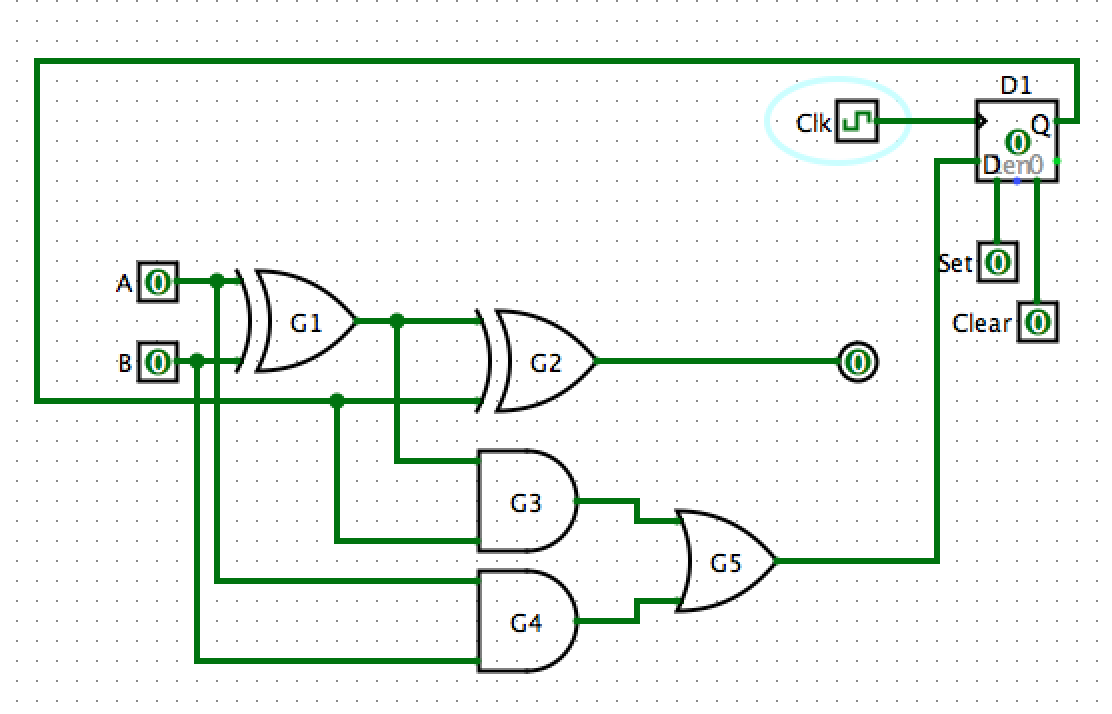
\includegraphics[scale=0.6]{sequential_carry_adder.png}
    \caption{Circuit of a Serial Adder}
\end{figure}

\emph{Definition File:}
\lstinputlisting{defn_files/sequential_carry_adder.txt}


\subsection{Binary Multiplier}
\begin{figure}[H]
    \centering
    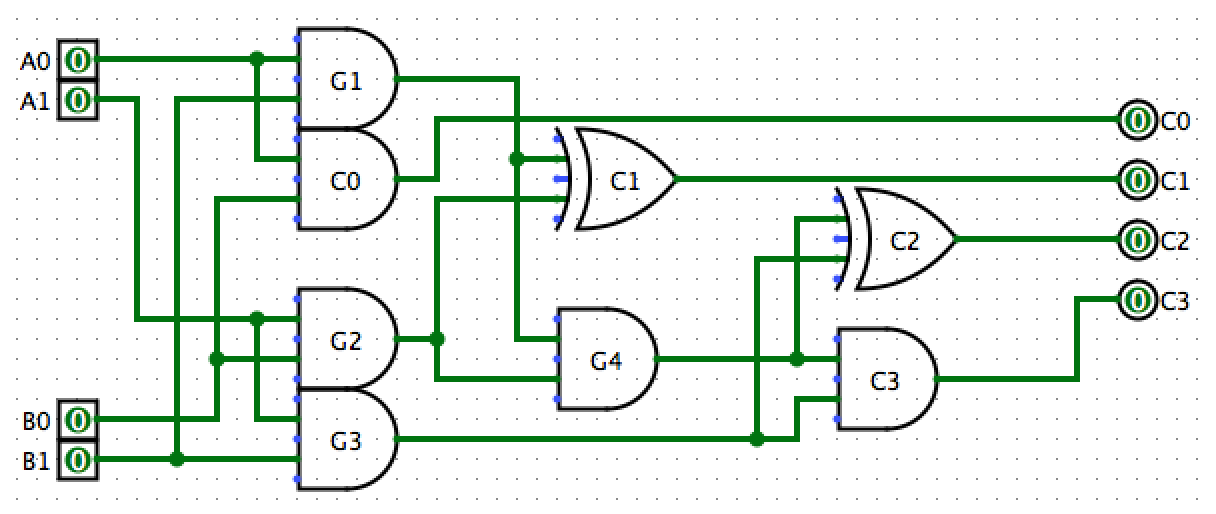
\includegraphics[scale=0.6]{bin_multiplier.png}
    \caption{circuit of a binary multiplier}
\end{figure}
\emph{Definition File:}
\lstinputlisting{defn_files/bin_multiplier.txt}


\end{document}
